\documentclass[tikz,border=10pt]{standalone}

\usetikzlibrary{calc}

\begin{document}
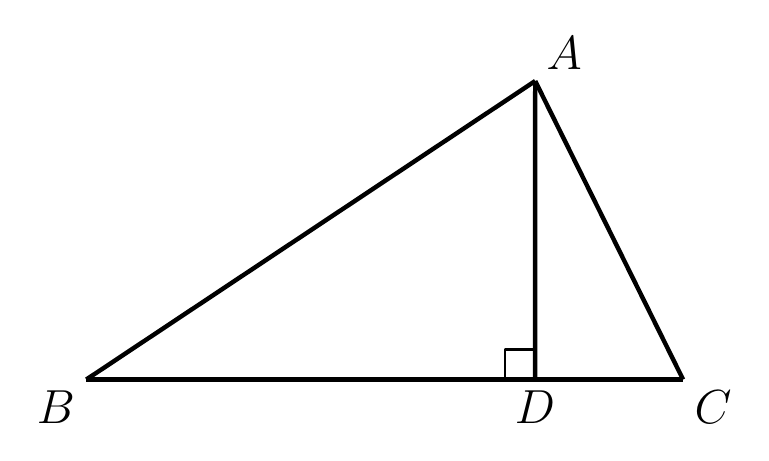
\begin{tikzpicture}[line join=round, line width=1.6pt,
  every node/.style={font=\fontsize{16.5}{19.8}\selectfont}]
\coordinate (A) at (1.891,1.902);
\coordinate (B) at (-3.810,-1.889);
\coordinate (C) at (3.769,-1.889);
\coordinate (D) at (1.889,-1.889);








\draw (A) -- (B);
\draw (A) -- (C);
\draw (B) -- (C);

\draw (A) -- (D);


\draw[line width=0.8pt] ($(D)+(0.000,0.380)$) -- ($(D)+(-0.380,0.380)$) -- ($(D)+(-0.380,0.000)$);


\node[above right] at (A) {$A$};
\node[below left] at (B) {$B$};
\node[below right] at (C) {$C$};
\node[below] at (D) {$D$};
\end{tikzpicture}
\end{document}